This result is motivated by the fact that being able to write $(A B)_H = A_H B_H$ allows to solve many problems. In particular, we could solve analytically (cf.\@~\autoref{app-analytic-exp}) many problems if it were the case.

"Multiplicity of the Heisenberg representation" refers to the fact that $(A B)_H = A_H B_H$. This appendix is presented in a way that mimics the reasoning that we followed. The appendix gives a good reason why the Heisenberg representation is non-multiplicative.

In this part, we find a sufficient condition for having $(A B)_H = A_H B_H$. To the best of our knowledge, this result is original. We limit ourselves to a time-independent Hamiltonian $H_S$ and to quantum jumps $\{L_\mu\}_\mu$. Beforehand, we introduce the notation
\begin{equation}
    \LS{A} \equiv \ihbar \commutator{A}{H_S} + \frac{1}{2} \sum_\mu \left( L^\dagger_\mu \commutator{A}{L_\mu}  - \commutator{A}{L^\dagger_\mu} L_\mu \right)
\end{equation}

which corresponds to the right hand side of the equation in~\autoref{eq_evo_heisen} before taking the Heisenberg representation, i.e.\@~$\timeDeriv{A_H} = \heis{\LS{A}}$.

We want to know whether $(A B)_H = A_H B_H$. Since at $t=0$, $(A B)_H(t=0) = A B = A_H(t=0) B_H(t=0)$, it suffices to show that $(A B)_H$ and $A_H B_H$ satisfy the same differential equation.

We start by writing the differential equations of $(A B)_H$ and of $A_H B_H$.
\begin{theorem}
    We have:
    \begin{eqnarray} \label{eq-diff-a-b}
        \timeDeriv{A_H B_H} &=& A_H \heis{\LS{B}} + \heis{\LS{A}} B_H\\ \label{eq-diff-(ab)}
        \timeDeriv{(A B)_H} &=& \heis{A \LS{B}} + \heis{\LS{A} B} + \sum_\mu \heis{\commutator{L^\dagger_\mu}{A} \commutator{B}{L_\mu}}
    \end{eqnarray}
\end{theorem}
We strongly encourage the reader to read the following proof since it is very instructive and gives a very good reason why $(A B)_H \neq A_H B_H$ in general.
\begin{proof}
On the one hand, we have:
\begin{equation}
    \timeDeriv{A_H B_H} = A_H \timeDeriv{B_H} + \timeDeriv{A_H} B_H = A_H \heis{\LS{B}} + \heis{\LS{A}} B_H
\end{equation}

On the other hand, we have:
\begin{eqnarray}
    \timeDeriv{(A B)_H} &=& \heis{\ihbar \commutator{A B}{H_S} + \frac{1}{2} \sum_\mu \left( L^\dagger_\mu \commutator{A B}{L_\mu}  - \commutator{A B}{L^\dagger_\mu} L_\mu \right)}\nonumber\\
    &=& \heis{\ihbar A \commutator{B}{H_S} + \frac{1}{2} \sum_\mu \left(\color{red} L^\dagger_\mu A \color{black} \commutator{B}{L_\mu}  - A \commutator{B}{L^\dagger_\mu} L_\mu \right)}\nonumber\\
    &+& \heis{\ihbar \commutator{A}{H_S} B + \frac{1}{2} \sum_\mu \left( L^\dagger_\mu \commutator{A}{L_\mu} B  - \commutator{A}{L^\dagger_\mu} \color{red} B L_\mu \color{black} \right)}
\end{eqnarray}

Before continuing the computation, we see that obtaining a quantity in the form $A ... + ... B$ that is expected from the product rule is prevented by the the presence of the jump operators on the right and on the left for $A$ and $B$ respectively. This confirms that the Heisenberg representation is non-multiplicative because of the jump operators. Let us try to put the product in the form $A ... + ... B$:
\begin{eqnarray}
    \timeDeriv{(A B)_H} &=& \heis{A \LS{B}} + \heis{\LS{A} B} + \frac{1}{2} \sum_\mu \heis{\commutator{L^\dagger_\mu}{A} \commutator{B}{L_\mu} - \commutator{A}{L^\dagger_\mu} \commutator{B}{L_\mu}}\nonumber\\
    &=& \heis{A \LS{B}} + \heis{\LS{A} B} + \sum_\mu \heis{\commutator{L^\dagger_\mu}{A} \commutator{B}{L_\mu}}
\end{eqnarray}
\end{proof}

From~\autoref{eq-diff-a-b} and~\autoref{eq-diff-(ab)}, we see that the difference between $(A B)_H$ and $A_H B_H$ is due to two facts. One the one hand, it is not guaranteed that $A_H \heis{\LS{B}} + \heis{\LS{A}} B_H = \heis{A \LS{B}} + \heis{\LS{A} B}$. One the other hand, the quantum jumps lead to the additional term in the evolution of $(A B)_H$, namely $\sum_\mu \heis{\commutator{L^\dagger_\mu}{A} \commutator{B}{L_\mu}}$.

One might be tempted to say that the sought condition is $\sum_\mu \heis{\commutator{L^\dagger_\mu}{A} \commutator{B}{L_\mu}} = 0$. Indeed, the counter-example in~\autoref{intro-heis-rep} does not satisfy this condition ($\commutator{a}{a^\dagger} \commutator{a^\dagger}{a} \neq 0$). However, we still need to show that $A_H \heis{\LS{B}} + \heis{\LS{A}} B_H = \heis{A \LS{B}} + \heis{\LS{A} B}$. We use the same strategy as before and write for eg.:

\begin{eqnarray}
    \timeDeriv{A_H \LS{B}} &=& A_H \heis{\LSS{2}{B}} + \heis{\LS{A}} \LS{B}\\
    \timeDeriv{(A \LS{B})_H} &=& \heis{A \LSS{2}{B}} + \heis{\LS{A} \LS{B}} + \sum_\mu \heis{\commutator{L^\dagger_\mu}{A} \commutator{\LS{B}}{L_\mu}}
\end{eqnarray}

with $f^{(n)}$ meaning the composition $n$ times. Therefore, we find that a sufficient condition that we would like to have is that $\sum_\mu \heis{\commutator{L^\dagger_\mu}{A} \commutator{\LS{B}}{L_\mu}} = 0$ and $A_H \heis{\LSS{2}{B}} + \heis{\LS{A}} \LS{B} = \heis{A \LSS{2}{B}} + \heis{\LS{A} \LS{B}}$. We start to see the inductive nature of the problem. Therefore, we introduce the following regularity condition:

\begin{definition}[Regularity condition]
    We say that the pair of operators $(A, B)$ is regular with respect to the quantum jumps $\{L_\mu\}_\mu$ when:
    \begin{equation}
        \forall r, s \in \mathbb{N}, \sum_\mu \heis{\commutator{L^\dagger_\mu}{\LSS{r}{A}} \commutator{\LSS{s}{B}}{L_\mu}} = 0
    \end{equation}
\end{definition}

Further, we introduce the sequence of propositions:

\begin{definition}[Sequence of propositions]
    For $n \in \mathbb{N}$, we introduce the proposition $\mathcal{P}(n)$:
    \begin{equation}
        \mathcal{P}(n) \equiv \left\{\forall r, s \in \mathbb{N}, r+s=n \implies \heis{\LSS{r}{A} \LSS{s}{B}} = \heis{\LSS{r}{A}} \heis{\LSS{s}{B}}\right\}
    \end{equation}
\end{definition}

We will show the following theorem:
\begin{theorem}[Sufficient condition if regularity]
    Under the \textbf{regularity condition}, we have:
    \begin{equation}
        \forall n \in \mathbb{N}, \mathcal{P}(n+1) \implies \mathcal{P}(n)
    \end{equation}
\end{theorem}

\begin{proof}
    Let $n \in \mathbb{N}$, let us suppose $\mathcal{P}(n+1)$.
    Let $r, s \in \mathbb{N}$, such that $r+s=n$, we have, using the regularity condition:
    \begin{equation}
        \timeDeriv{\heis{\LSS{r}{A} \LSS{s}{B}}} = \heis{\LSS{r+1}{A} \LSS{s}{B}} + \heis{\LSS{r}{A} \LSS{s+1}{B}}
    \end{equation}
    Since $(r+1)+s = r+(s+1) = n+1$, applying the proposition $\mathcal{P}(n+1)$, we can write:
    \begin{eqnarray}
        \timeDeriv{\heis{\LSS{r}{A} \LSS{s}{B}}} &=& \heis{\LSS{r+1}{A}} \heis{\LSS{s}{B}} + \heis{\LSS{r}{A}} \heis{\LSS{s+1}{B}}\nonumber\\ 
        &=& \timeDeriv{\left[\heis{\LSS{r}{A}} \heis{\LSS{s}{B}}\right]}
    \end{eqnarray}
    Therefore: $\heis{\LSS{r}{A} \LSS{s}{B}} = \heis{\LSS{r}{A}} \heis{\LSS{s}{B}}$, which shows $\mathcal{P}(n)$.
\end{proof}

We can represent the structure that we uncovered using a reverse Pascal triangle~\cite{wiki-pascal-triangle}, cf.\@~\autoref{fig:image-pascal}.

\begin{center}
    \begin{figure}[h!]
      \centering
      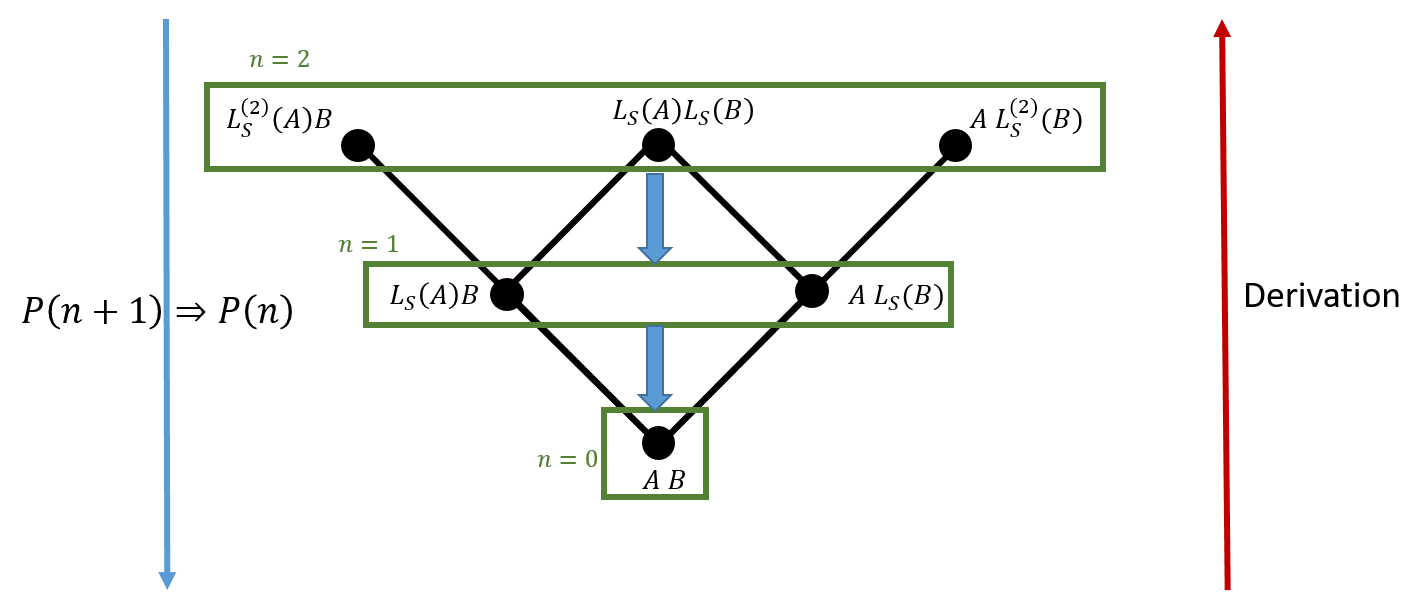
\includegraphics[width=0.9\linewidth]{Pics/image-pascal.png}
      \caption{Inverse Pascal triangle structure that appears under the regularity condition for the pair of operators $(A, B)$. Deriving corresponds to creating two upwards branches to the left (derive $A$) and to the right (derive $B$). The implication $\mathcal{P}(n+1) \implies \mathcal{P}(n)$ goes downwards.}
      \label{fig:image-pascal}
    \end{figure}
\end{center}